\section{Neuronale Netze}
Ein Neuron ist ein Schwingkreis. Es hat n Eingänge und einen Ausgang. Die Werte der
Eingänge werden summiert. Wenn die Summe der Eingänge einen Schwellwert übertrifft, wechselt der Ausgang, das Neuron feuert.
Für die Schwellwertfunktion, wird entweder die Signum (0/1) oder die Sigmoid-Funktion welche ``weiche'' Kanten hat und ableitbar ist verwendet.
\begin{figure}[htb]
	\centering
	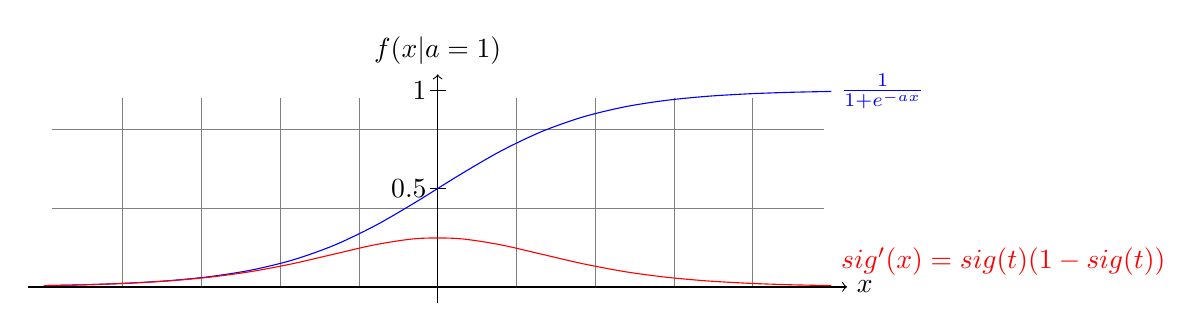
\begin{tikzpicture}[domain=-5:5, smooth, samples=20]
	\draw[very thin, color=gray] (-4.9,0.0) grid (4.9,2.4);

	\draw[->] (-5.2,0) -- (5.2,0) node[right] {$x$};
	\draw[->] (0,-0.2) -- (0,2.7) node[above] {$f(x|a=1)$};
	\draw (-0.1,2.5) --(0.1,2.5) node [left] {$1~$};
	\draw (-0.1,1.25) -- (0.1,1.25) node [left] {$0.5~$};

	\draw[color=blue] plot (\x,{2.5 / (1+exp(-\x))}) node[right] {$\frac{1}{1+e^{-ax}}$};
	\draw[color=red]  plot (\x,{2.5 / (1+exp(-\x)) * (1-1/(1+exp(-\x)))}) node[above right] {$sig'(x)=sig(t)(1-sig(t))$};
\end{tikzpicture}


	\caption{Sigmoid Funktion mit a=1}
\end{figure}
\subsection{Übersicht}
\begin{table}[htbp]
	\setlist{nolistsep}
	\centering
	\begin{tabular}{l | p{8cm}}
		Typ & Merkmale \\
		\hline
		{klassisches Perzeptron} & {
			\begin{itemize}
				\item Können nur linear separierbare Probleme lösen
				\item Ein einzelnes Perzeptron-Neuron kann 14 Schnittebenen legen
			\end{itemize}
		}
		\\
		{Holographisches Perzeptron} & {
			\begin{itemize}
				\item Verwendet Komplexe Zahlen
				\item Sehr grosse Speicherfähigkeit
				\item Grosse Verarbeitungsgeschwindigkeit
				\item Stochastische Resonanz (benötigt Rauschen im Input)
			\end{itemize}
		}
		\\
		{Kohonen-Netze} & {
			\begin{itemize}
				\item Topographisches Netz
				\item Geeignet für TSP-Problem
			\end{itemize}
		}
		\\
		{Hopfield} & {
			\begin{itemize}
				\item Lernt nicht bzw. unüberwachtes Lernen
				\item Nur eine Schicht, gleichzeitig Ein- und Ausgabe
				\item Jedes der binären Neuronen mit jedem verbunden
				\item Erkennt invertierte Muster als gleich
			\end{itemize}
		}
	\end{tabular}
	\caption{Vergleich zwischen verschiedenen Neuronalen Netzen}
	\label{tab:nnetze}
\end{table}
\subsection{Klassisches Neuron / Perzeptron}
Das Perzeptron ist das klassische mathematische Neuron. Es besteht aus:
\begin{itemize}
	\item Summierer
	\item Feuerschwelle
	\item Ausgabefunktion (Sigmoid)
\end{itemize}
\subsection{Netze elementarer Perzeptronen}
\subsection{Backpropagation}
\subsection{Holographisches Perzeptron}
\subsection{Kohonennetze}
Kohonennetze sind selbstorganisierend. Sie bestehen aus aneinandergereiten Neuronen, mit variablen Abstand (Gummiband).
\subsubsection{Beispiel Travelling Salesman}
\begin{itemize}
	\item Neuronen zufällig platzieren
	\item Auswahl zufälliger Stadt
	\item Das am nächsten liegende Neuron nehmen und näher zu dieser Stadt rücken, die anderen Neuronen nachziehen
	\item Wiederholen bis alle Neuronen ihren Platz gefunden haben
\end{itemize}
\subsection{Hopfield}
Das Hopfield-Netz ist geeignet um Muster (Bilder) zu kennen. Dabei wird pro Pixel ein binäres Neuron verwendet (-1,1).
Dazu erstellt man eine Korrelationsmatrix, welche alle Muster enthält, es wird nicht gelernt!
Pro zu erkennendes Muster werden etwa 7 Neuronen benötigt.
Für eine gute Erkennung sollten die Muster möglichst orthogonal, also linear unabhängig sein.

